\section{Subtyping, Polymorphie und Vererbung}
\subsection{Konzepte}
\subsubsection{Subtyping}
\begin{multicols}{2}
	Subtyping beschreibt das Konzept einer Typhirarchie. \texttt{Exp} repräsentiert Algemeine Ausdrücke. Jedes \texttt{Literal}, aber auch jede \texttt{Addition} ist ein \texttt{Exp}.\\ 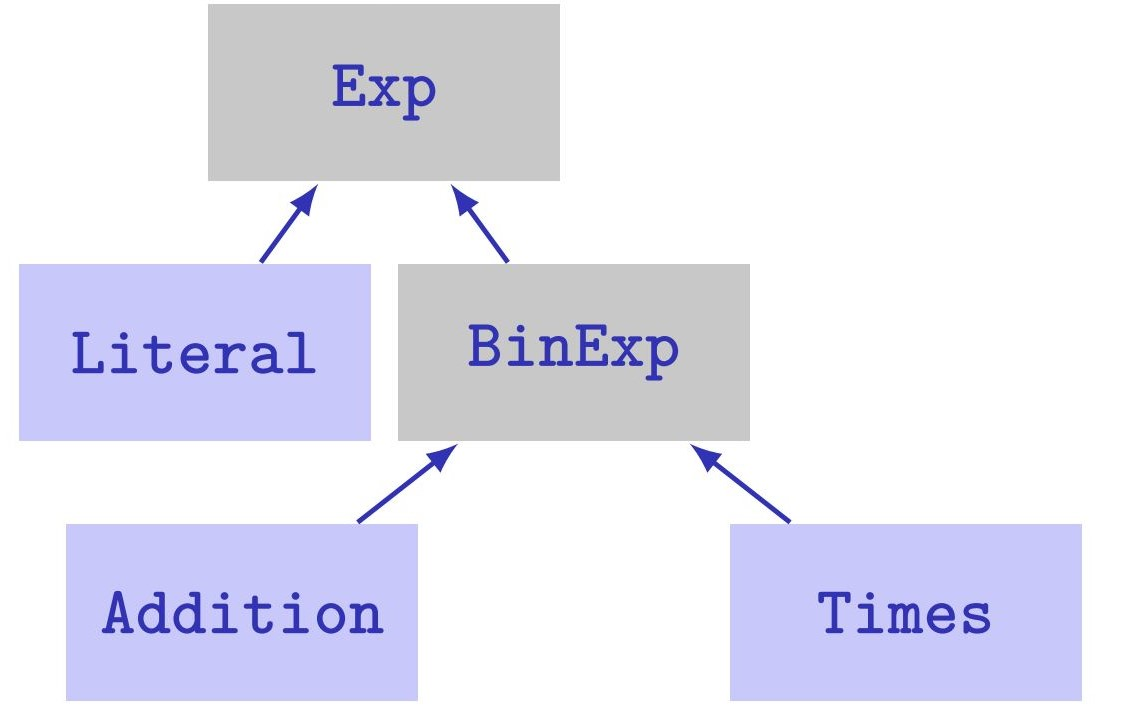
\includegraphics[width=0.12 \textwidth]{sections/subtyping}
\end{multicols}
Überall wo ein \texttt{Exp} erwartet wird, kann auch \texttt{Literal} oder \texttt{Times} genutzt werden.
\subsubsection{Polymorphie und dynamische Bindung}
Eine Variable vom statiscen Typ \texttt{Exp} kann Ausdrücke mit unterschiedlichen dynamischen Typen ''beherbergen''. Ausgeführt werden die Memeberfunktionen des dynamischen Typs.
\begin{lstlisting}
	Exp* e = new Literal(2);
	std::cout<< e->eval(); // 2
	
	e = new Addition(e,e);
	std::cout<< e->eval(); // 4 (eval von Addtion)
\end{lstlisting}
\subsubsection{Vererbung}
Manche Funktionalitäten sind für mehrere Mitglider der Typhirarchie gleich. Zum Codeduplikation zu verhindern die Funktion an Subtyp vererben.
\begin{lstlisting}
	class Exp{...};
	class BinExp : public Exp{...};
	class Times : public BinExp{...};
\end{lstlisting}
\texttt{BinExp} ist eine Subklasse von \texttt{Exp} und eine Superklasse von \texttt{Times}.
\subsection{Anwendung}
\begin{lstlisting}
	class Exp{
		public:
		virutal int size() const = 0;
		virutal double eval() const = 0;
	};
	class Literal : public Exp{
		double val;
		public:
		Literal(double v);
		int size() const;
		double eval() const;
	};
\end{lstlisting}
\texttt{Exp} ist ein abstrakte Klasse. \texttt{=0} erzwingt die Implementierung in der Subklasse. \texttt{virtual} aktiviert die Dynamische Bindung.\\
\texttt{Literal} erbt durch \texttt{public Exp} von \texttt{Exp} ist sonst aber eine normale Klasse.
Bei virtuellen Memberfunktionen bestimmt der dynamische Typ die auszuführende Memberfunktion (dynamische Bindung)  ohne virtual der statische Typ.
Gemeinsamkeiten von \texttt{Times} und \texttt{Addtion} können in \texttt{BinExp} ausgelagert werden.
\begin{lstlisting}
	class BinExp : public Exp{
		Exp* left;
		Exp* right;
		public:
		BinExp(Exp* l, Exp* r);
		int size() const;
	};
	BinExp::BinExp(Exp* l, Exp* r) : left(l), right(r) {}
	int BinExp::size() const {
		return 1 + this->left->size() + this->right->size();
	}
\end{lstlisting}
\texttt{BinExp} implementiert \texttt{eval()} nicht und ist darum auch eine abstrakte Klasse. Die Gemeinsamkeiten von \texttt{BinExp} werden weriterverwerbt.
\begin{lstlisting}
	class Addition : public BinExp {
		public:
		Addition(Exp* l, Exp* r);
		double eval() const;
	};
	Addition::Addition(Exp* l, Exp* r) : BinExp(l,r){}
	double Addition::eval() const{
		return this->left->eval() + this->left->eval();
	}
\end{lstlisting}
\texttt{Addition} erbt die Membervariabeln \texttt{left}, \texttt{right} und die Funktion \texttt{size} von \texttt{BinExp}. Genau genommen hat \texttt{Addition} jedoch kein Zugriff auf \texttt{left} und \texttt{right}, da diese \texttt{privat} sind in \texttt{BinExp}. \texttt{BinExp} bräuchte eine Memberfunktion, die \texttt{left} und \texttt{right} zurückgibt und somit den Zugriff gewährt. \todo{Das ist schon so oder???}




